%%%%%%%%%%%%%%%%%%%%%%%%%%%%%%%%%%%%%%%%%%%%%%%%%%%%%%%%%%%%%%%%%%%%%%%%%%%%%%%%
%2345678901234567890123456789012345678901234567890123456789012345678901234567890
%        1         2         3         4         5         6         7         8

\documentclass[letterpaper, 10 pt, conference]{ieeeconf}  % Comment this line out if you need a4paper

%\documentclass[a4paper, 10pt, conference]{ieeeconf}      % Use this line for a4 paper

\IEEEoverridecommandlockouts                              % This command is only needed if 
                                                          % you want to use the \thanks command

\overrideIEEEmargins                                      % Needed to meet printer requirements.

% See the \addtolength command later in the file to balance the column lengths
% on the last page of the document

% The following packages can be found on http:\\www.ctan.org
%\usepackage{graphics} % for pdf, bitmapped graphics files
%\usepackage{epsfig} % for postscript graphics files
%\usepackage{mathptmx} % assumes new font selection scheme installed
%\usepackage{times} % assumes new font selection scheme installed
%\usepackage{amsmath} % assumes amsmath package installed
%\usepackage{amssymb}  % assumes amsmath package installed



\usepackage{amsmath,amssymb}

\usepackage{tikz,hyperref,graphicx,units,subfig}
\usepackage{benktools}

\usepackage{sidecap,wrapfig}
\usepackage[ruled,vlined]{algorithm2e}
\DeclareMathOperator*{\argmin}{arg\,min}
\DeclareMathOperator*{\argmax}{arg\,max}
\newcommand{\abs}[1]{\lvert#1\rvert} 
\newcommand{\norm}[1]{\lVert#1\rVert}
%\newcommand{\suchthat}{\mid}
\newcommand{\suchthat}{\ \big|\ }
\newcommand{\bd}{\mathbf{d}}
\newcommand{\bn}{\mathbf{n}}
\newcommand{\bp}{\mathbf{p}}
\newcommand{\bw}{\mathbf{w}}
\newcommand{\by}{\mathbf{y}}
\newcommand{\bx}{\mathbf{x}}
\newcommand{\bz}{\mathbf{z}}
\newcommand{\bbf}{\mathbf{f}}
\newcommand{\bzero}{\mathbf{0}}
\newcommand{\bG}{\mathbf{G}}
\newcommand{\bA}{\mathbf{A}}
\newcommand{\bW}{\mathbf{W}}
\newcommand{\bX}{\mathbf{X}}
\newcommand{\mX}{\mathcal{X}}
\newcommand{\mD}{\mathcal{D}}
\newcommand{\mN}{\mathcal{N}}
\newcommand{\mW}{\mathcal{W}}
\newcommand{\mF}{\mathcal{F}}
\newcommand{\bZ}{\mathbf{Z}}

\newcommand{\bfc}{W}
\newcommand{\Qinf}{Q_{\infty}}
\newcommand{\st}[1]{_\text{#1}}
\newcommand{\rres}{r\st{res}}
\newcommand{\pos}[1]{(#1)^+}
\newcommand{\depth}{\operatorname{depth}}
\newcommand{\dist}{\operatorname{dist}}
\newcommand{\convhull}{\operatorname{ConvexHull}}
\newcommand{\minksum}{\operatorname{MinkowskiSum}}



\title{\LARGE \bf
Efficient Sampling for Grasp Quality Evaluation with Gaussian Process Implicit Surface Representation }


\author{Michael Laskey, Zoe McCarthy, Florian T. Pokorny, Jeff Mahler, Sachin Patil,\\ Danica Kragic, Jur Van Den Berg, Pieter Abbeel, and Ken Goldberg}% <-this % stops a space

\newtheorem{theorem}{Theorem}

\begin{document}



\maketitle
\thispagestyle{empty}
\pagestyle{empty}


%%%%%%%%%%%%%%%%%%%%%%%%%%%%%%%%%%%%%%%%%%%%%%%%%%%%%%%%%%%%%%%%%%%%%%%%%%%%%%%%



%%%%%%%%%%%%%%%%%%%%%%%%%%%%%%%%%%%%%%%%%%%%%%%%%%%%%%%%%%%%%%%%%%%%%%%%%%%%%%%%
\section{Introduction}

\vspace{10pt}

\todo{Write a better Intro, needs to have a better sell}
Many modern 3d sensors give noisy point clouds as output, so shape uncertainty is a common problem \cite{singhbigbird}. As shown in Fig. \ref{fig:noisy data}, the noise in our measurements of object shape can greatly change the surface normals and contact points, which are the parameters that most grasp metrics rely on.  A number of metrics have been proposed to evaluate form and force closure with scalar quality measures for grasping \cite{bicchi2000}.   However, only recently have people started looking into a metric's robustness to uncertainty. 
 
We use Gaussian Processes \cite{rasmussen2006} to convert the point cloud measurements into an implicit surface with uncertainty in the shape. Gaussian Processes provide a formal way to incorporate uncertainty, however this sophisticated representation presents new challenges for evaluating the expected grasp quality. The wrench-space Ferrari-Canny force closure quality measure \cite{ferrari1992} calculates the maximum disturbance that can be resisted given bounds on the contact forces.

We assume that a robot's $m$ grippers approach the grasped object along straight lines (which we call lines of action), and analyze how this grasping model interacts with the probability distribution on shapes described by a Gaussian Process Implicit Surface (GPIS).
We calculate and visualize the theoretical probability distributions on grasp contact points and normals and the expected center of mass induced by the GPIS and line of action.
Then demonstrate how sampling from this explicit grasp distribution can be used to reduce the complexity associated with Monte-Carlo integration of the expected grasp quality over the distribution of shapes. 

We also treat the problem of finding the best grasp in a set of proposed grasps as a n-arm bandit problem and propose an $\epsilon$ - greedy policy for finding the best grasp in the set in an anytime like manner. 

\begin{figure}[ht!]
\centering
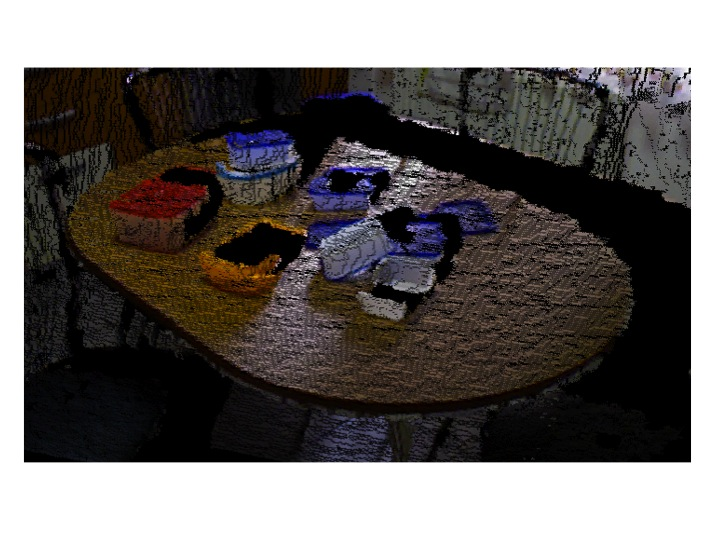
\includegraphics[scale = 0.3]{figures/Slide02.jpg}
\caption{An example of the noise from a Kinect-like sensor}
\vspace*{-10pt}
\label{fig:noisy data}
\end{figure}

\todo{Get an actual Kinect Image}

\section{Related Work}

While a variety of grasp metrics have been proposed, few explicitly looked at uncertainty in grasp parameters. Zheng et al. looked at friction and contact point uncertainty \cite{zheng2005}. He computed the maximum distance a contact point was allowed to deviate from its expected grasp, while maintaining force closure. Kehoe et al. looked at shape uncertainty for push grasps, however this was limited to parallel jaw grippers and only measured the probability of force closure \cite{kehoe2012toward}. More closely related to our approach is the work of Christopoulos and Schrater \cite{christopoulos2007handling}. They use a spline representation for uncertainty and measure the probability of losing force closure, their approach though is limited to two contacts. Our method looks at not only force closure, but provides the quality of the expected grasp and an upper bound on the expexted change from that quality. 

The choice of using a Gaussian Process Implicit Surface to represent our uncertainty, stems from the fact that it provides a formal way to include various sources of noise in observations. Prior work has used uncertainty representation such as independent Gaussian noise on each vertex in a Polygonal mesh \cite{kehoe2012toward}. However, this doesn't provide a continuous function one can easily compute distributions on grasp parameters with. GPIS is also becoming more prevalent in the grasping community with recent work by Dragiev et al. \cite{dragiev2011} . The utilization of uncertainity around an implicit surface allows us to compute explicit distributions on contacts and surface normals, which to our knowledge has not been done formally. 

\todo{Write about n-arm bandit literature}

\section{Gaussian Process Implicit Surfaces}

In this section we describe the mathematical derivation of Gaussian Process Implicit Surface representations.

\subsection{Gaussian Process (GP) Background}

Gaussian processes (GPs) are widely used in machine learning as a nonparametric regression method for estimating continuous functions from sparse and noisy data \cite{rasmussen2010gaussian}.
In a GP, a training set consists of input vectors $\mX = \{\bx_1, \ldots, \bx_n\}$, $\bx_i \in \mathbb{R}^d$, and corresponding observations $\by = \{y_1, \ldots, y_n\}$. The observations are assumed to be noisy measurements from the unknown target function $f$:
\begin{equation}
y_i = f(\bx_i) + \epsilon,
\end{equation}
where $\epsilon \sim \mN(0,\sigma^2)$ is Gaussian noise in the observations.
A zero-mean Gaussian process is completely specified by a covariance function $k(\cdot,\cdot)$, also referred to as a kernel.
Given the training data $\mD = \{\mX, \by\}$ and covariance function $k(\cdot,\cdot)$, the posterior density $p(f_*|\bx_*,\mD)$ at a test point $\bx_{*}$ is shown to be \cite{rasmussen2010gaussian}:
\begin{align}
	p(f_*|\bx_*,\mD) &\sim \mN\big(\mu(\bx_*), \Sigma(\bx_*)\big) \label{eq:GPposterior} \\
	\mu(\bx_*) &= k(\mX,\bx_*)^{\intercal}(K + \sigma^2I)^{-1}\by \label{eq:GPmean} \\
	\Sigma(\bx_*) &= k(\bx_*,\bx_*)-k(\mX,\bx_*)^{\intercal}(K+\sigma^2I)^{-1}k(\mX,\bx_*)\big) \label{eq:GPvar}
\end{align}
where $K \in \mathbb{R}^{n \times n}$ is a matrix with entries $K_{ij} = k(\bx_i,\bx_j)$ and $k(\mX,\bx_*) = [k(\bx_1,\bx_*),\ldots,k(\bx_n,\bx_*)]^{\intercal}$. 
This derivation can also be used to predict the mean and variance of the function gradient by extending the kernel matrices using the identities \cite{solak2003derivative}:

\begin{align*}
	\text{cov}\left(f(\bx_i), f(\bx_j) \right) &=  k(\bx_i, \bx_j) \\
	\text{cov}\left(\frac{\partial f (\bx_i)}{\partial x_k}, f(\bx_j) \right) &= \frac{\partial}{\partial x_k} k(\bx_i, \bx_j) \\
	\text{cov}\left(\frac{\partial f (\bx_i)}{\partial x_k}, \frac{\partial f (\bx_j)}{\partial x_l} \right) &= \frac{\partial^2}{\partial x_k \partial x_l} k(\bx_i, \bx_j)
\end{align*}

\subsection{Kernel Selection}
The choice of kernel is application-specific, since the function $k(\bx_i,\bx_j)$ is used as a measure of correlation between states $\bx_i$ and $\bx_j$. A common choice is the squared exponential kernel:
\begin{equation}
	k(\bx_i,\bx_j) = \nu^2\exp(-\frac{1}{2}(\bx_i - \bx_j)^{\intercal}\Lambda^{-1}(\bx_i - \bx_j))
\end{equation}
where $\Lambda= \text{diag}(\lambda_1^2,\ldots,\lambda_d^2)$ are the characteristic length scales of each dimension of $\bx$ and $\nu^2$ describes the variability of $f$.
Other common kernels relevant to GPIS are the thin-plate splines kernel \cite{williams2007} and the Matern kernel \cite{bjorkman2013enhancing}.

The measurement noise parameter $\sigma$ is usually estimated based on a model of the sensor used to collect measurements
The vector of remaining hyperparameters $\boldsymbol{\theta} = \{\nu, \lambda_1,\ldots,\lambda_d\}$ is optimized during the training process by maximizing the log-likelihood $p(\by|\mX,\boldsymbol{\theta})$, usually using gradient descent \cite{rasmussen2010gaussian}.
The log-likelihood function is subject to local maxima, and therefore the hyperparamter search often involves a search over the maxima found from several random initializations of the hyperparamters.



\begin{figure}[ht!]
\centering
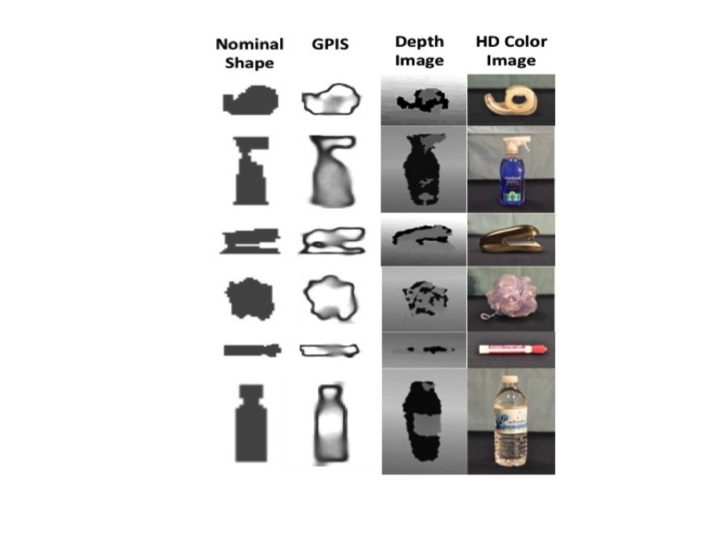
\includegraphics[scale = 0.3]{figures/Slide03.jpg}
\caption{Left: A surface represented as a Truncated Signed Distance Field (TSDF).
Right: A GPIS reconstruction from noisy samples of the left surface's TSDF.}
\vspace*{-10pt}
\label{fig:GPIS_TSDF}
\end{figure}
%\section{Related Work}


\section{Problem Definition}

%The objective of our algorithm is to provide a quality of the expected grasp, $Q_l^-(\bar{g})$ \cite{ferrari1992}, and a lower bound $b$ that is the expected deviation from the quality of the expected grasp. 

We assume a bounded 2-d rectangular workspace $\mathcal{R}$.
We parameterize a single grasp $g$ on an object with the following tuple $g = ( \textbf{c}_1,...,\textbf{c}_m,\textbf{n}_1,...,\textbf{n}_m,\textbf{z},\tau )$.
We have an indexing set $I$ of $m$ point contacts and surface normal on the object: for $i \in I$ the contact is located at $c_i$ with surface normal $n_i$.
The object has a center of mass $z$ and friction coefficient $\tau$.
The line segment $\gamma(\cdot)$ has endpoints $a,b$ that are defined as the start of the gripper and the intersection of the line with the end of the workspace respectively, as shown in Fig. 
 \ref{fig:line_of_action}.


We assume that the robot grippers move along the line of action until they make contact with the object and stop.
Since we have uncertainty in the shape this induces a distribution on the grasp parameters subject to the line, hence $p(g) = ( p(\textbf{c}_1),...,p(\textbf{c}_m),p(\textbf{n}_1),...,p(\textbf{n}_m),\bar{\textbf{z}},\tau )$.
We note that $\tau$ is considered known and $\bar{z}$ is the expected center of mass, not a full probability distribution. In section \ref{sec:distgrasp}, we demonstrate how to efficiently compute the distributions on contact points and surface normals and expected center of mass. 




\section{Distribution of Grasp Parameters}
\label{sec:distgrasp}

 For the following derivations we introduce the following,
 $\theta(x) = ( \mu(x),\Sigma(x) )$, where $\theta(x)$ is a tuple consisting of the mean and covariance functions given by the trained GPIS model \cite{rasmussen2006} . 
 
 To calculate $p(g)$, we assume a gripper contacts approaches along a parameterized line of action, or a 1-dimensional curve in the work space, defined by $\gamma(t)$. See Fig \ref{fig:line_of_action}, for a detailed illustration. Each gripper contact is defined by a line of action, so we assume the following tuple is provided $\Gamma = ( \gamma_1(\cdot),...,\gamma_m(\cdot) )$, these approach trajectories are then used to compute a distribution on grasp parameters. 
 



 %We also define the  level set function as $f(x): \mathbb{R}^d \rightarrow \mathbb{R}$ and an implicit surface as $\mathcal{S} = \{ x \ | \ f(x) = 0 \}$.

\todo{Get a better figure for line of action model}


\begin{figure}[ht!]
\centering
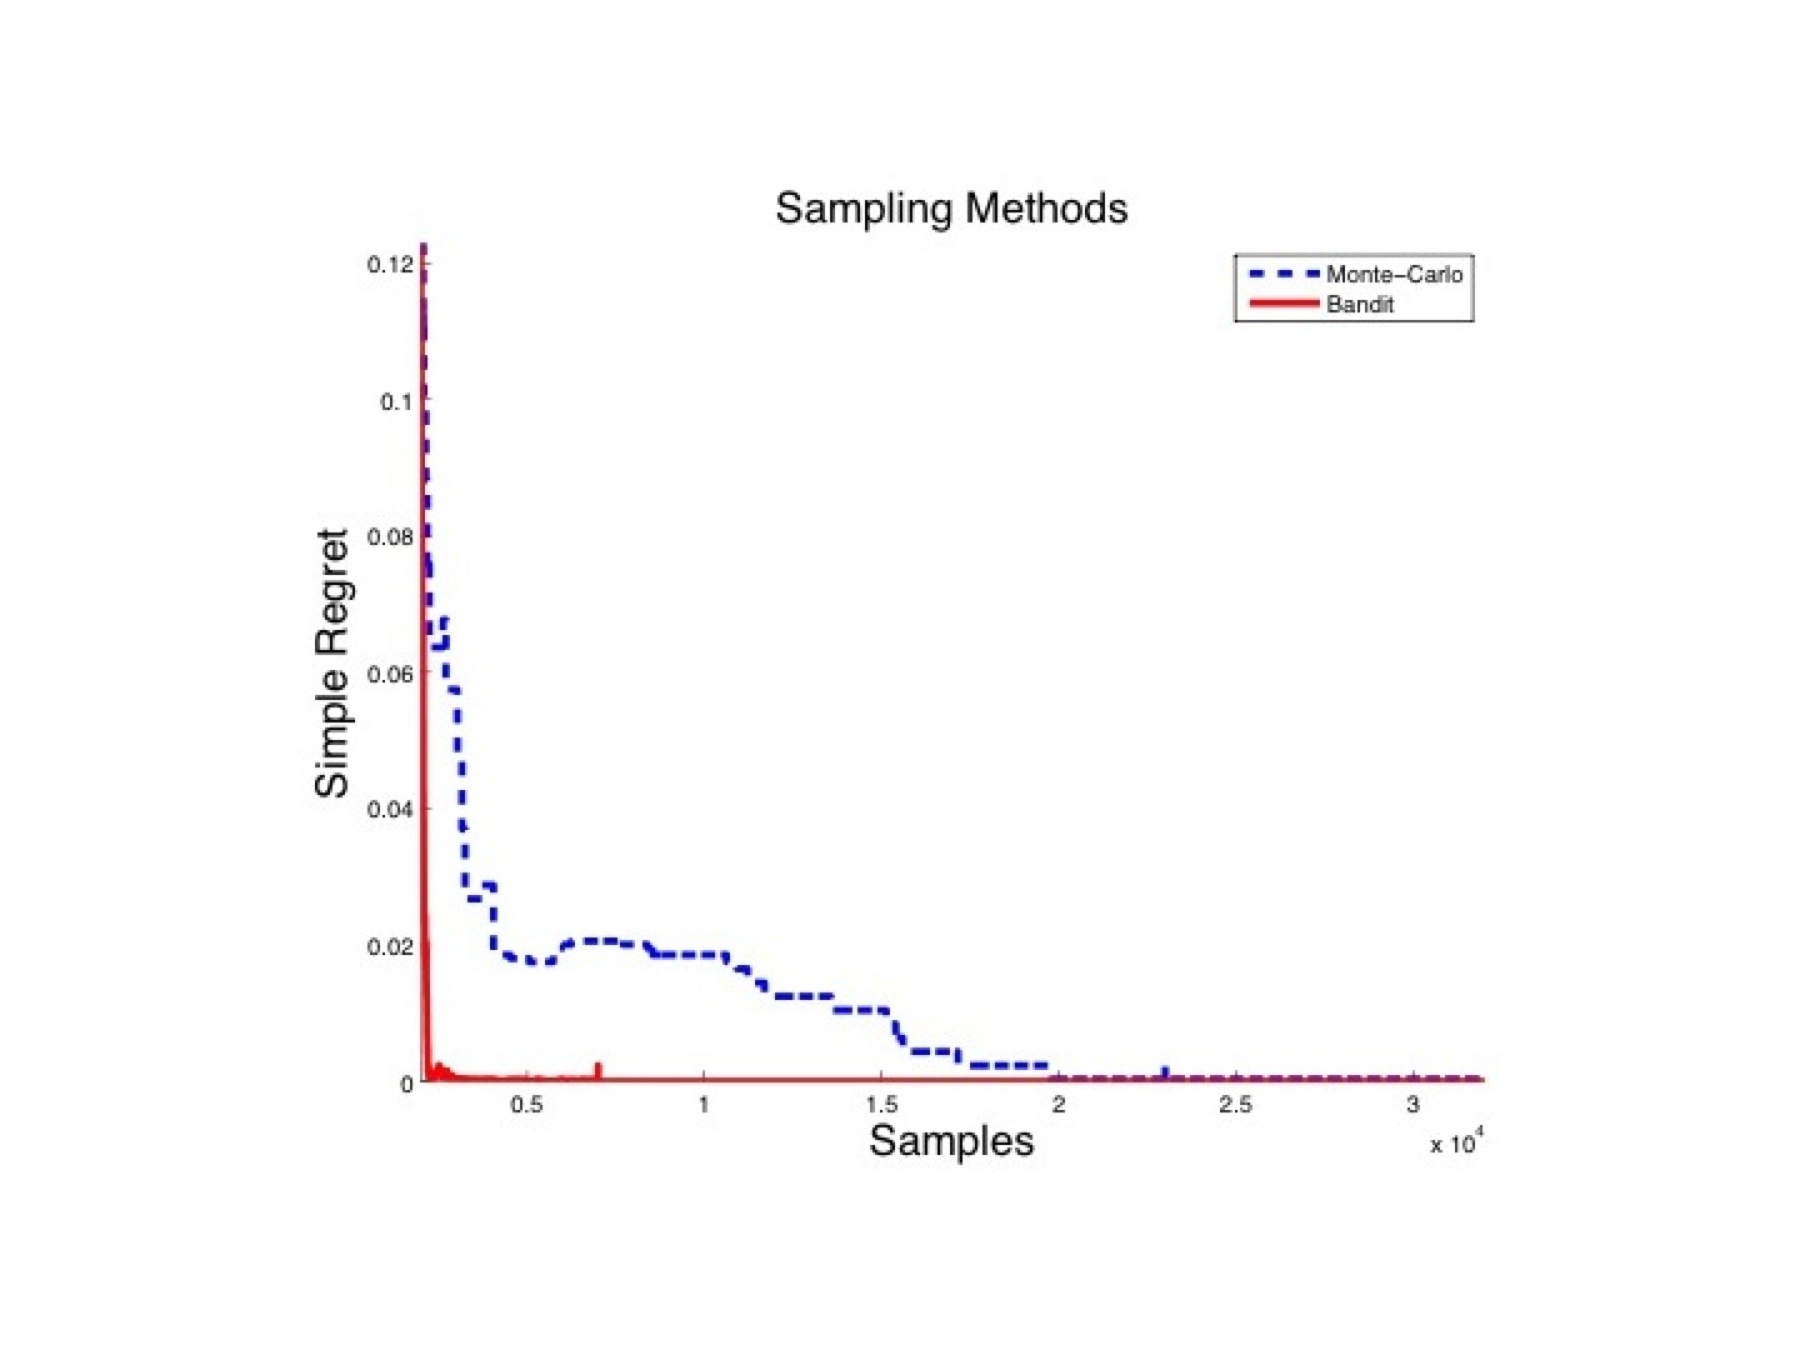
\includegraphics[scale = 0.3]{figures/Slide01.jpg}
\caption{Parameterized Line of Action along an object}
\vspace*{-10pt}
\label{fig:line_of_action}
\end{figure}
%\textbf{TODO:MORE DESCRIPTIVE GRAPHIC}
\subsection{Distribution on Contact Points} 
In our implementation we discretize along the line $\gamma(t)$ evenly but write the derivation in continuous form for generality.
The probability distribution along the line $\gamma(t)$ is given by the following:

\begin{equation}
p\big(f(\gamma(t))|\theta(\gamma(t)): \forall t \in [a,b] \big) 
=
\mN(\mu_{a:b},\Sigma_{a:b}).
\end{equation}

This gives the signed distance function distributions along the entire line of action in the workspace as a multivariate gaussian.
We would like to find the distribution on the first contact point, which we can define as when the signed distance function $f(\gamma(t))$ is $0$ and all previous times $\tau$ we have $f(\gamma(\tau)) > 0$ for $0 \leq \tau < t$.
This ensures $t$ is at the edge of the surface (having $f(\gamma(t)) = 0$) and that for all previous $\tau$ the gripper was outside of the surface (having $f(\gamma(\tau)) > 0$).
We thus compute this as the joint distribution $p\big(\textbf{c}_i= \gamma(t)\big) = p\big(f(\gamma(t))=0, f(\gamma(\tau))> 0: \forall \tau \in [0,t)\big)$.
%Hence we want to know at a point what the distribution  is that it is at the surface and the probability that all points before are before the surface,
This avoids the problem of the distribution producing multiple modes along the line: one for each intersection with the surface.
We now derive this distribution 

\[
  p\big(\textbf{c}_i = \gamma(t)\big) \propto 
\]
\[
  p\big(f(\gamma(t)) = 0\big)P\big(f(\gamma(\tau)) > 0 | f(\gamma(t)) = 0: \forall \tau \in [0,t)\big)
\]

where we only indicate proportionality and will later normalize to probability $1$.
Using the first product in the equation can be computed easily using the marginalization of a multivariate Gaussian distribution and the second one can be rewritten by conditioning the distribution \cite{petersen2008matrix}. 

\begin{align*}
p_c\big(f(\gamma(\tau)): \forall \tau \in [0,t)\big) = p\big(f(\gamma(\tau))  | f(\gamma(t)) = 0\big)  
\end{align*}


The following can now be said:

\[
  p\big(\textbf{c}_i = \gamma(t)\big) = 
\]
\[
  = \frac{1}{\eta} p(f(\gamma(t)) = 0) P_c\big(f(\gamma(\tau)) > 0): \forall \tau \in [0,t)\big)			 
\]

for the appropriate $\eta$ normalization factor.
The second product term can be evaluated by calculating the cumulative distribution of a multivariate Gaussian, which we calculate with the Matlab function $mvncdf$.
We show again the theoretical distribution on $\textbf{c}_i$ calculated for a given GPIS and approach direction in Fig.
\ref{fig:GraspContactPt}.
%efficiently evaluated by looking up the cumulative distribution of a multivariate Gaussian, which is common in most software packages \cite{matlab}.

\begin{figure}[ht!]
\centering
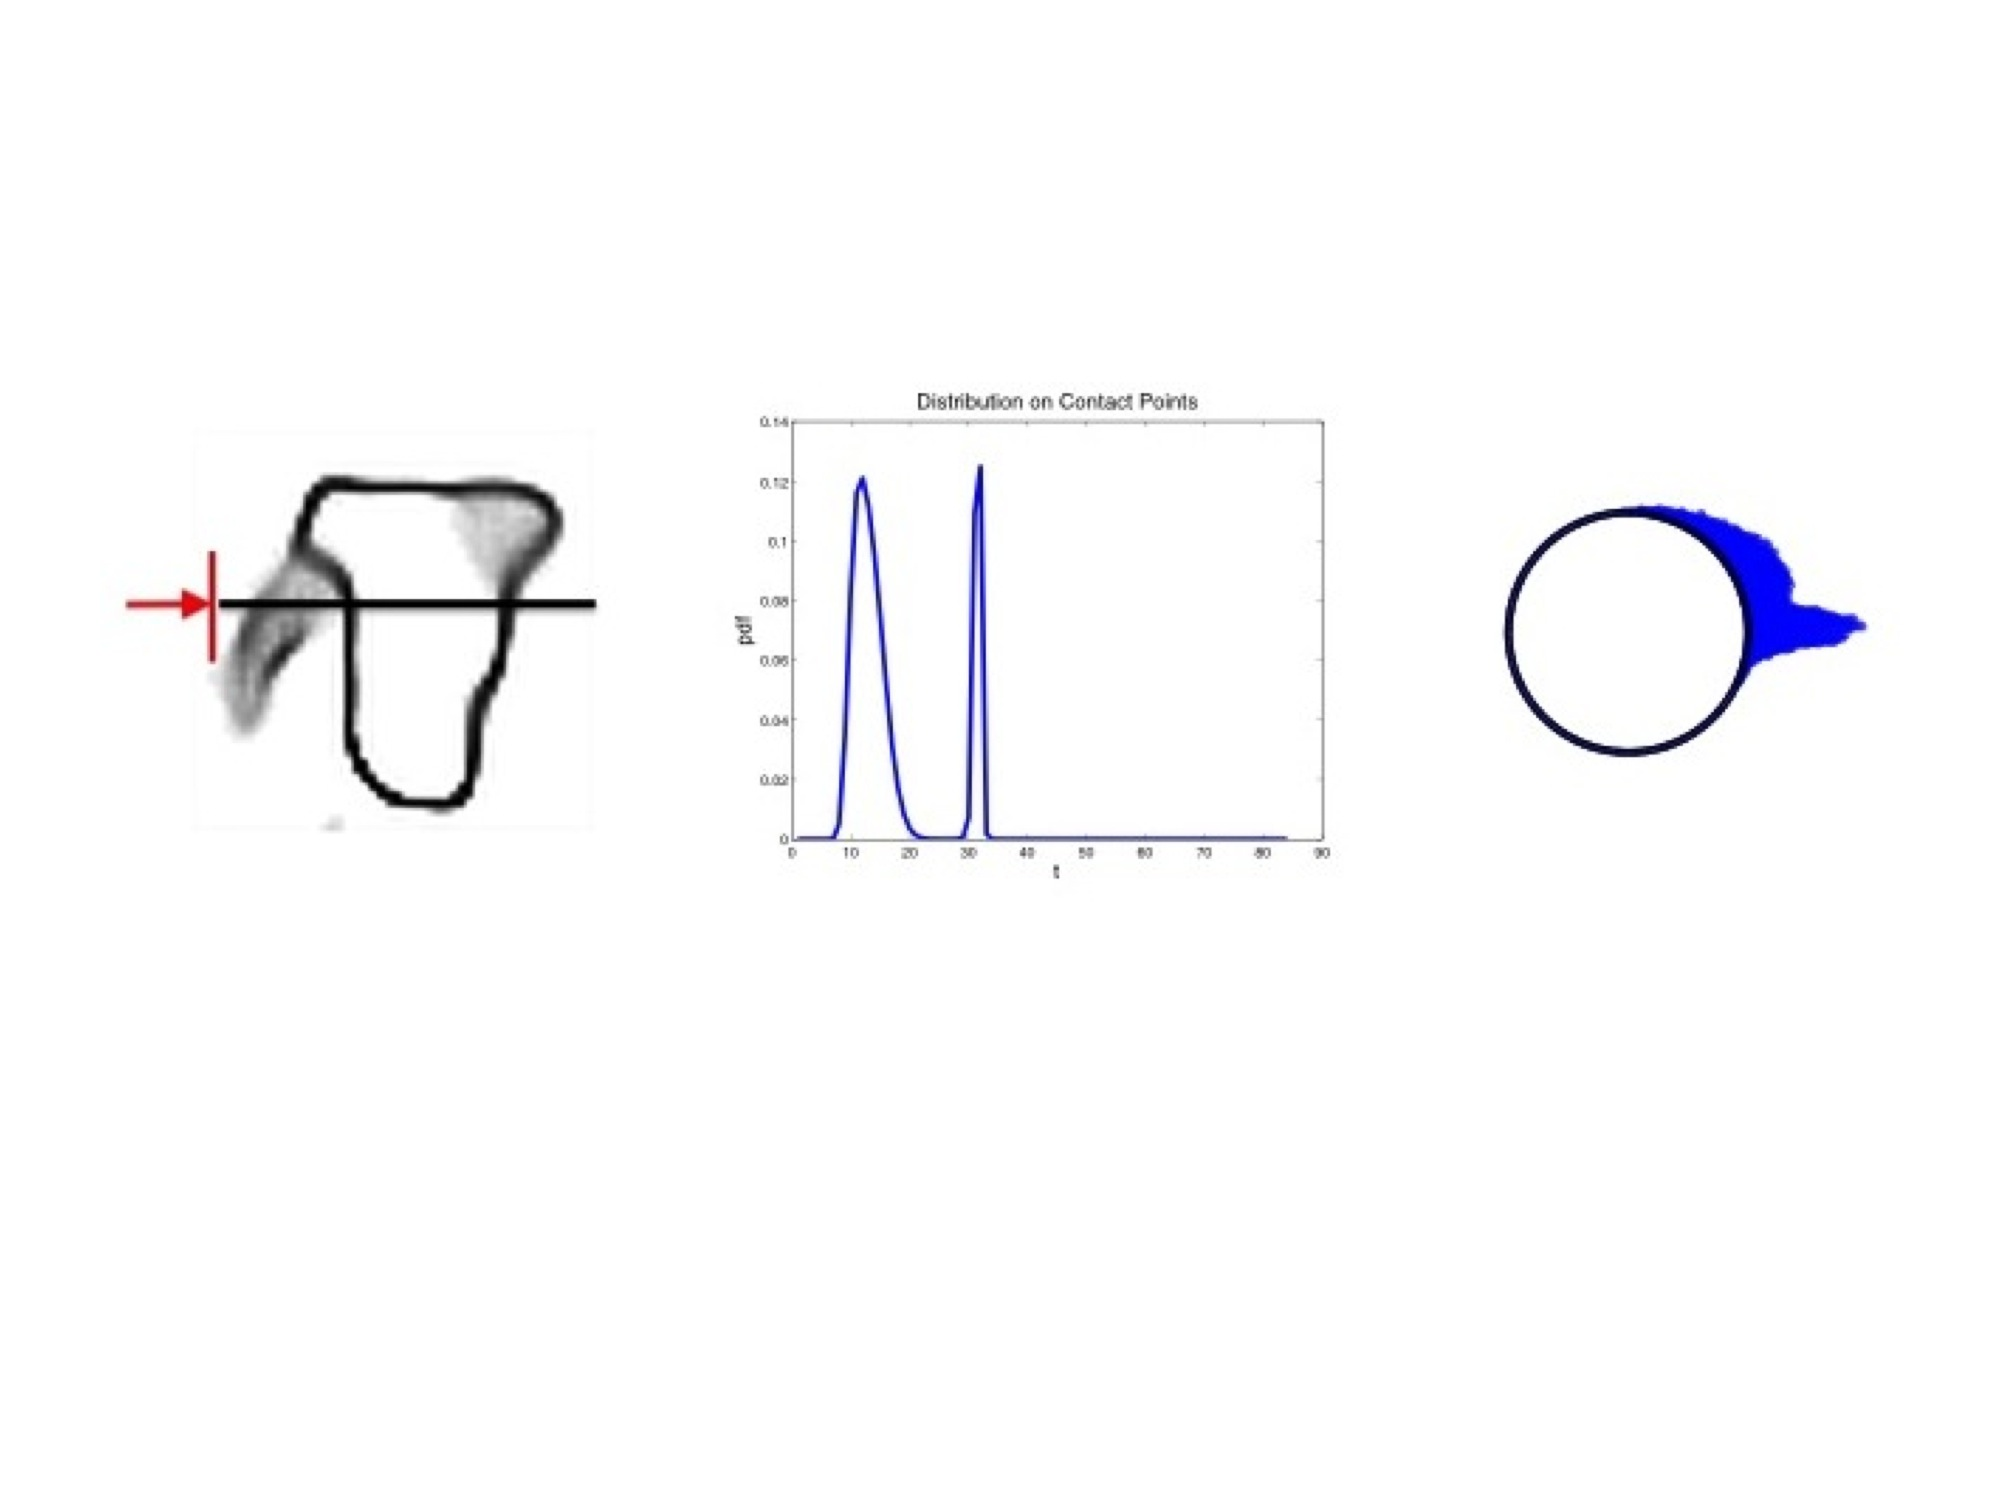
\includegraphics[scale = 0.3]{figures/Slide04.jpg}
\caption{Left: Grasp approach direction on an uncertain surface, represented by a Gaussian Process Implicit Surface.  Right: Induced distribution on the contact point as a function of x-axis position along the approach line.}
\vspace*{-10pt}
\label{fig:GraspContactPt}
\end{figure}

\subsection{Distribution on Surface Normals} 
The distribution of surface normals $p(\textbf{n}_i = \textbf{v})$ can be calculate as follows.
First we assume that some function exists $h(x) = ( \mu_{\nabla}(x), \Sigma_{\nabla}(x) )$, hence given a point $\bf{x}$ it returns the parameters for a Gaussian distribution around the gradient.
this function can be computed via learning the gradient \cite{solak2003derivative} or analytical differentiation of $f(x)$.
We note that both methods yield a Gaussian distribution.
We now demonstrate how to marginalize out the contact distribution and compute $p(\textbf{n}_i = \textbf{v})$.\\

From our distribution on contact points and Bayes rule we can compute the following: 

\begin{equation}
p(\textbf{c}_i = \gamma(t), \textbf{n}_i = \textbf{v}) = p\big(\textbf{n}_i = \textbf{v} | \textbf{c}_i = \gamma(t) \big)p\big(\textbf{c}_i = \gamma(t)\big)
\end{equation}

Now we can marginalize out the distribution on contacts:

\begin{equation}
p(\textbf{n}_i = \textbf{v}) = \int_a^b  p \big(\textbf{n}_i = \textbf{v} | \textbf{c}_i = \gamma(t) \big)p(\textbf{c}_i = \gamma(t)) dt
\end{equation}

\begin{equation}
p\big(\textbf{n}_i = \textbf{v}\big) = \int_a^b  p \big(\textbf{n}_i = \textbf{v} | h(\gamma(t))\big)p\big(\textbf{c}_i = \gamma(t)\big) dt
\end{equation}

We approximate this by uniformly sampling the integral along the function $\gamma(t)$ and achieve the following: 

\begin{equation}
p\big( \textbf{n}_i = \textbf{v} \big) = \sum_T  p \big( \textbf{n}_i = \textbf{v} | h(\gamma(t)) \big) p\big(\textbf{c}_i = \gamma(t)\big) \Delta t
\end{equation}


Grasp metrics such as  Ferrari-Canny require $\textbf{n}_i$ be normalized, or, equivalently, a member of $\mathcal{S}^{d-1}$ \cite{ferrari1992}. To account for this we project the Gaussian distribution $p \big(\textbf{n}_i = \textbf{v} |\textbf{c}_i = \gamma(t) \big)$  onto $\mathcal{S}^{d-1}$. We use a projection technique developed by Olano and North \cite{olano1997normal}. In Fig.
\ref{fig:GraspSurfaceNormals}, we show the theoretical distribution on $\textbf{n}_i$ calculated for a given GPIS and approach direction.

\begin{figure}[ht!]
\centering
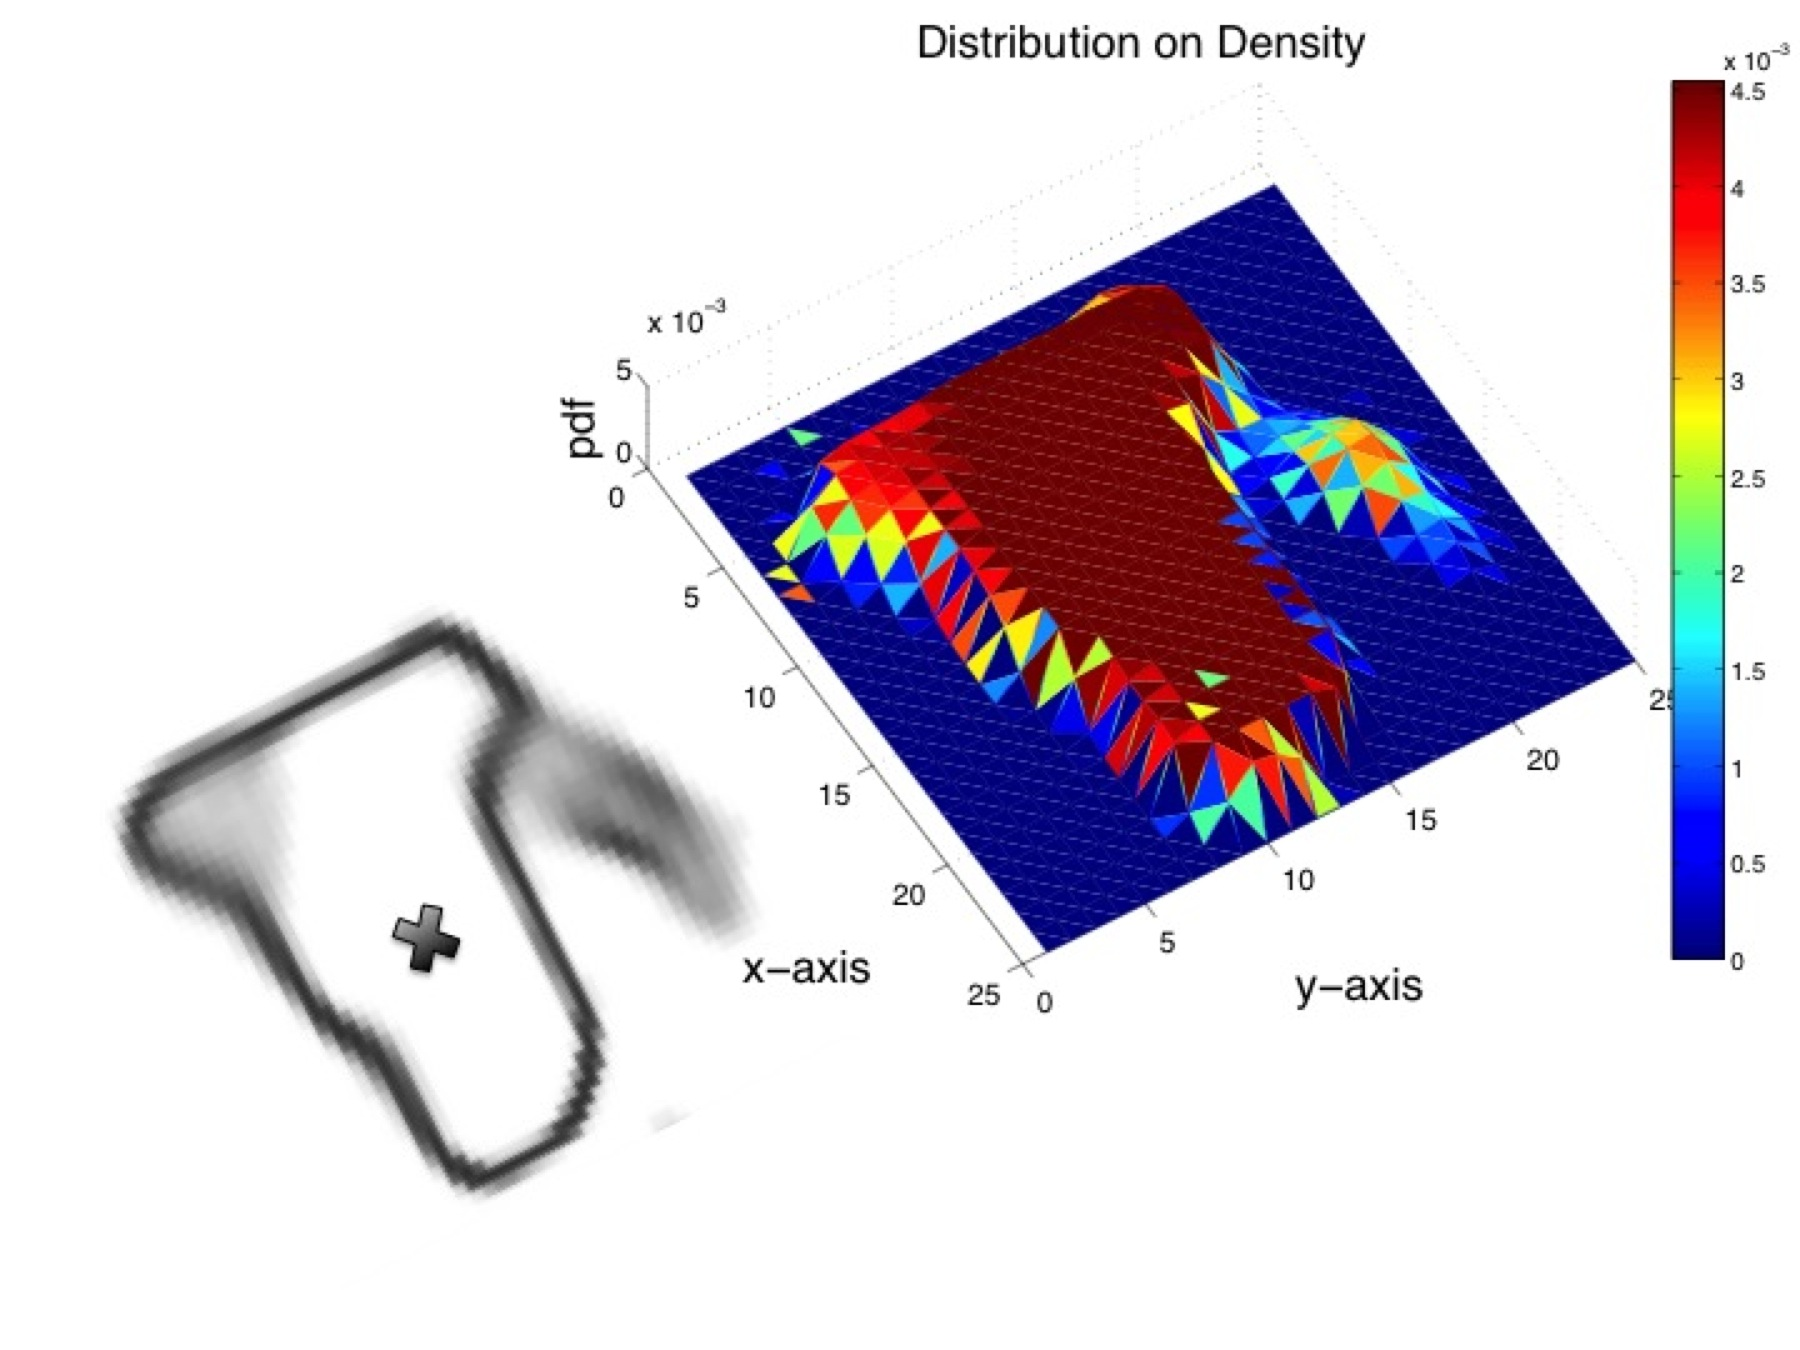
\includegraphics[scale = 0.3]{figures/Slide05.jpg}
\caption{Left: Grasp approach direction on an uncertain surface, represented by a Gaussian Process Implicit Surface.
Right: Induced distribution on the surface normals.}
\vspace*{-10pt}
\label{fig:GraspSurfaceNormals}
\end{figure}

\subsection{Expected Center of Mass} 

We recall the quantity CDF$(f(x))(0) = \int_{-\infty}^{0} p(f(x) =  s \ | \ \theta(x)) ds$ as the cumulative distribution function of $f(x)$ evaluated at 0 and note that it is equal to the probability that $x$ is interior to the surface under the current observations.
We assume that the object has uniform mass density and then CDF$(f(x))(0)$ is the expected mass density at $x$.
Then we can find the expected center of mass as:

\begin{equation}
  \bar{z} 
  =
  \frac
    {\int_{\mathcal{R}}x CDF(f(x))(0) dx}
    {\int_{\mathcal{R}}  CDF(f(x))(0) dx}
\end{equation}

which can be approximated by sampling $\mathcal{R}$ uniformly in a grid and approximating the spatial integral by a sum. We show the computed density and calculated expected center of mass for a marker in Fig. \ref{fig:GPIS_MASS}.


\begin{figure}[ht!]
\centering
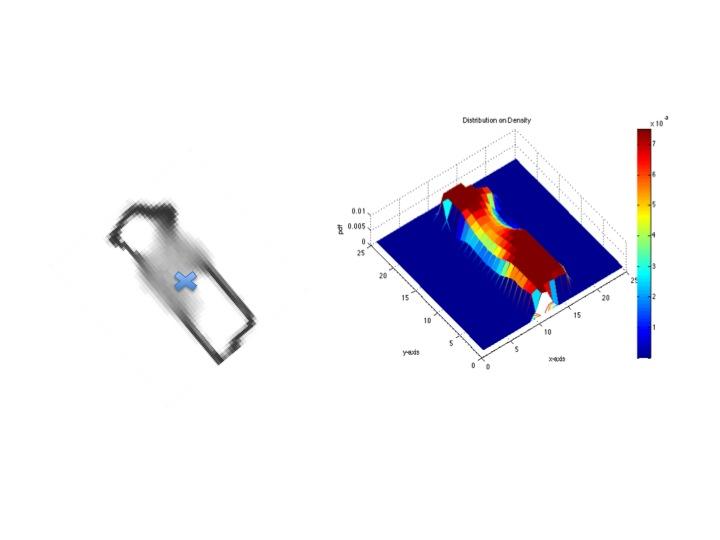
\includegraphics[scale = 0.3]{figures/Slide06.jpg}
\caption{Left: A surface with GPIS construction and expected center of mass (blue X)
Right: The distribution on the density of each point assuming uniform center of mass}
\vspace*{-10pt}
\label{fig:GPIS_MASS}
\end{figure}

\section{Sampling from a GPIS}
Prior work that consider shape uncertainty purposed sampling from distribution on the shape itself \cite{kehoe2012toward}. However, with a more complicated model on the shape distribution this technique would scale poorly. 

Given a work space $\mathcal{R}^{n\times n}$, the complexity of sampling a work space is show to be $O(n^6)$. This is due to the necessary inversion of a $n \times n$. In typical cases $n$ would be on the order of 100 making this very computationally intensive even in the 2D case. 

If we instead sample from our proposed grasp distributions and use a line of action that is roughly equal to $n$, the complexity can be rewritten as $O(T*n^3)$,  where $T$ is the number of grasps that are evaluated. 


\section{Adaptive Sampling for Grasp Selection}
In a possible grasping scenario, one would be presented with a set $G$ of $T$ grasps. The goal would be to identify, which one is the best grasp given the set $G$ and for each grasp the $p(g)$. While a naive approach to solving this problem would be to simply perform Monte-Carlo integration on each one and compute the expected grasp quality, we propose treating the problem as an n-arm bandit problem and forming a policy for selecting which grasp to sample. The motivation behind this is due to the expensive evaluation that each Ferrari-Canny computation takes \cite{ferrari1992}.

An n-arm bandit problem can be defined as follows: an agent is presented with a $n$ slot machines and receives a reward each time a lever is pulled that is drawn from the distribution associated with the slot machine. The goal of the agent is to maximize the expected reward received, by balancing exploration and exploitation \cite{barto1998reinforcement}.

For selecting grasps we use an $\epsilon$-greedy policy, where the greedy action is selected with probability $1-\epsilon$ and a random action is chosen otherwise. The greedy option is defined as the grasp with the highest approximate upper confidence bound $v$, which is computed via the following \cite{mc} 

\begin{equation}
v = \bar{X} + \frac{1.96 \bar{\sigma}_N}{\sqrt{n}}
\end{equation}






\section{Experiments}

\subsection{Validation of Grasp Distributions}

To validate our theoretical calculations, we compared them to empirical distributions found via Monte-Carlo Sampling. The qualitative results for surface normals and contacts can be found in Figures \ref{fig:Contact_Dist} and \ref{fig:Normal_Dist} respectively. We present the numerical comparison with KL-divergence in Table 1, as you can see the distributions are very closely related. 

\begin{table}[h]
        \begin{tabular}{ l | c c c}
         Distribution & \bf Marker & \bf Tape & \bf Loofa \\ 
        \hline \\
         p($\textbf{c}_i$) & 0.14 & 0.08 & 0.02 \\
        \hline \\
        p($\textbf{n}_i$)& 0.35 & 0.12 & 0.16 \\
        \hline 
        \end{tabular}
        \caption{The KL-Divergence for different distributions on the contact points and surface normals}
		
        \vspace*{-10pt}
\end{table}


\begin{figure}[h]
\centering
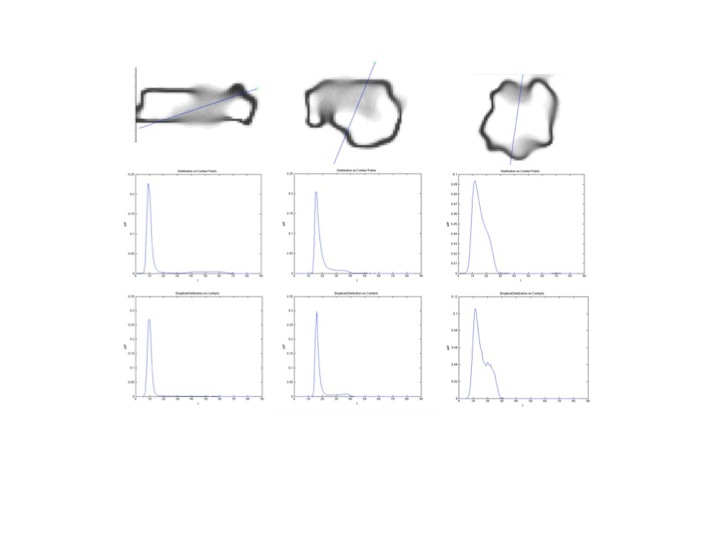
\includegraphics[scale = 0.3]{figures/Slide07.jpg}
\caption{Top: A surface with GPIS construction and line of action with the start pointed denoted by green x.
Middle: Theoretical distribution computed on contact point
Bottom: Empirically sampled distribution}
\vspace*{-10pt}
\label{fig:Contact_Dist}
\end{figure}

\begin{figure}[ht!]
\centering
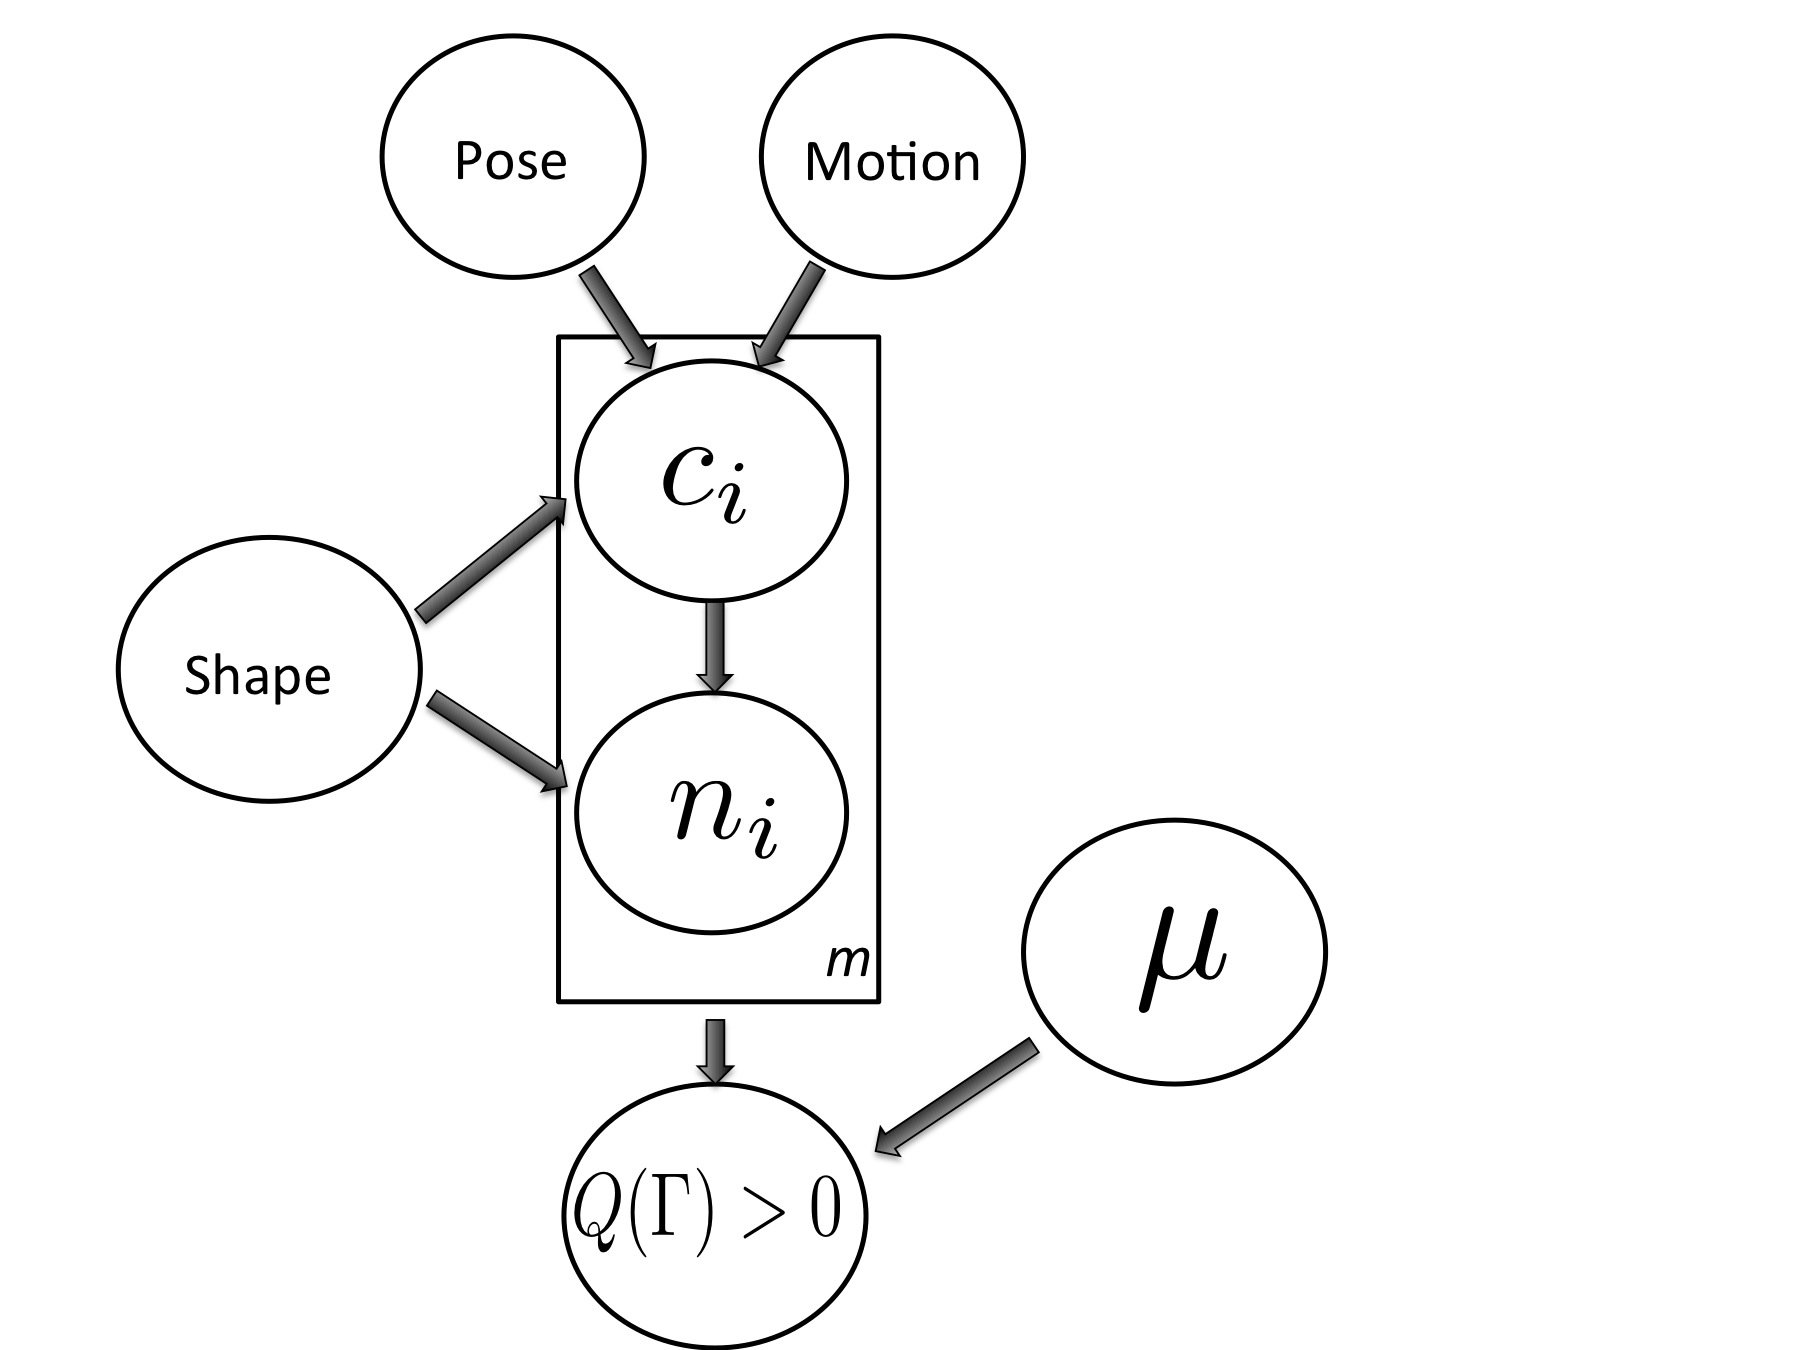
\includegraphics[scale = 0.3]{figures/Slide08.jpg}
\caption{Top: A surface with GPIS construction and line of action with the start pointed denoted by green x.
Middle: Theoretical distribution computed for surface normals
Bottom: Empirically sampled distribution}
\vspace*{-10pt}
\label{fig:Normal_Dist}
\end{figure}

\subsection{Sampling from Grasps Vs. Shape}
We first demonstrate that sampling from the two different method converges to near the same expected value, see Fig. \ref{fig:sampling_convergence}. After confirming the distributions converge to the same value we show the computational complexity in Fig. \ref{fig:speed_dif} of the two methods for evaluating 100 grasps on an $n \times n$ grid. 

\begin{figure}[ht!]
\centering
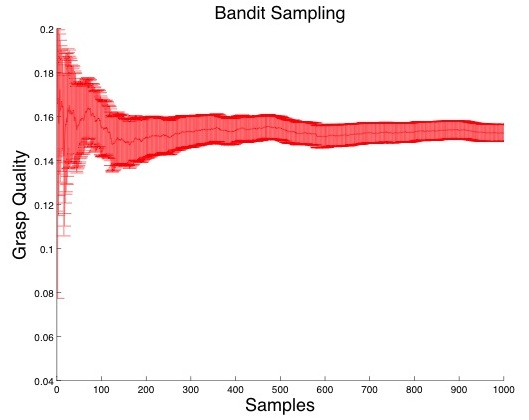
\includegraphics[scale = 0.3]{figures/Slide11.jpg}
\caption{Left: Sampling from grasp distributions
Right: Sampling from distribution on shape}
\vspace*{-10pt}
\label{fig:sampling_convergence}
\end{figure}

\begin{figure}[ht!]
\centering
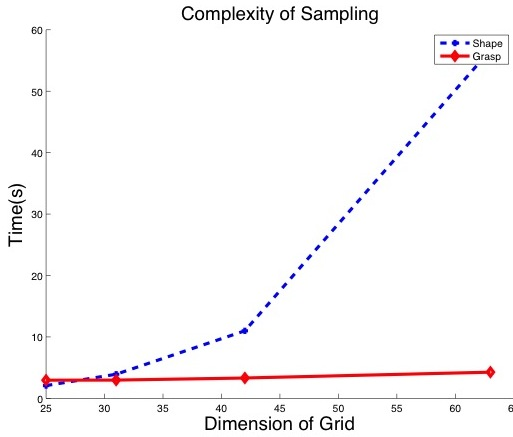
\includegraphics[scale = 0.3]{figures/Slide12.jpg}
\caption{Comparison of the computational complexity of the two methods with respect to the work space dimensions}
\vspace*{-10pt}
\label{fig:speed_dif}
\end{figure}

\subsection{Adaptive Sampling Technique}

We consider the problem of selecting the best grasp out of a set $G$ given a fix number of iterations $I$. For our experiments we look at selecting the best grasp out of a size of $|G| = 100$ and given a fix iteration limit of $I = 1000$. We show the results for both the marker and tape, in Fig. \ref{fig:marker_bandit} and Fig. \ref{fig:tape_bandit} respectively. We note that in both cases the policy was able to select the best grasp without sufficiently sample the set of possible grasps. 

\todo{Add experiments demonstrating ordering and trials over large number of runs, also fix visualizations}

\begin{figure}[ht!]
\centering
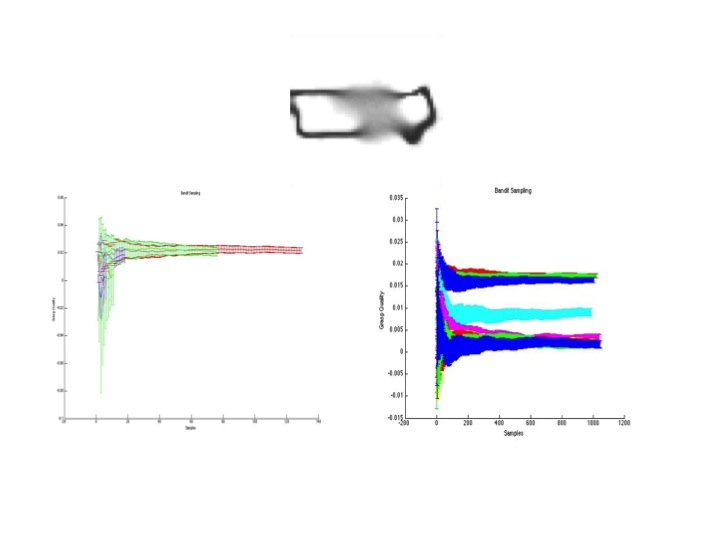
\includegraphics[scale = 0.3]{figures/Slide09.jpg}
\caption{Left: $\epsilon$-greedy policy for sampling (Top 10 grasps plotted)
Right: Monte-Carlo Sampling for 1000 iterations (Top 10 grasps plotted)}
\vspace*{-10pt}
\label{fig:marker_bandit}
\end{figure}


\begin{figure}[ht!]
\centering
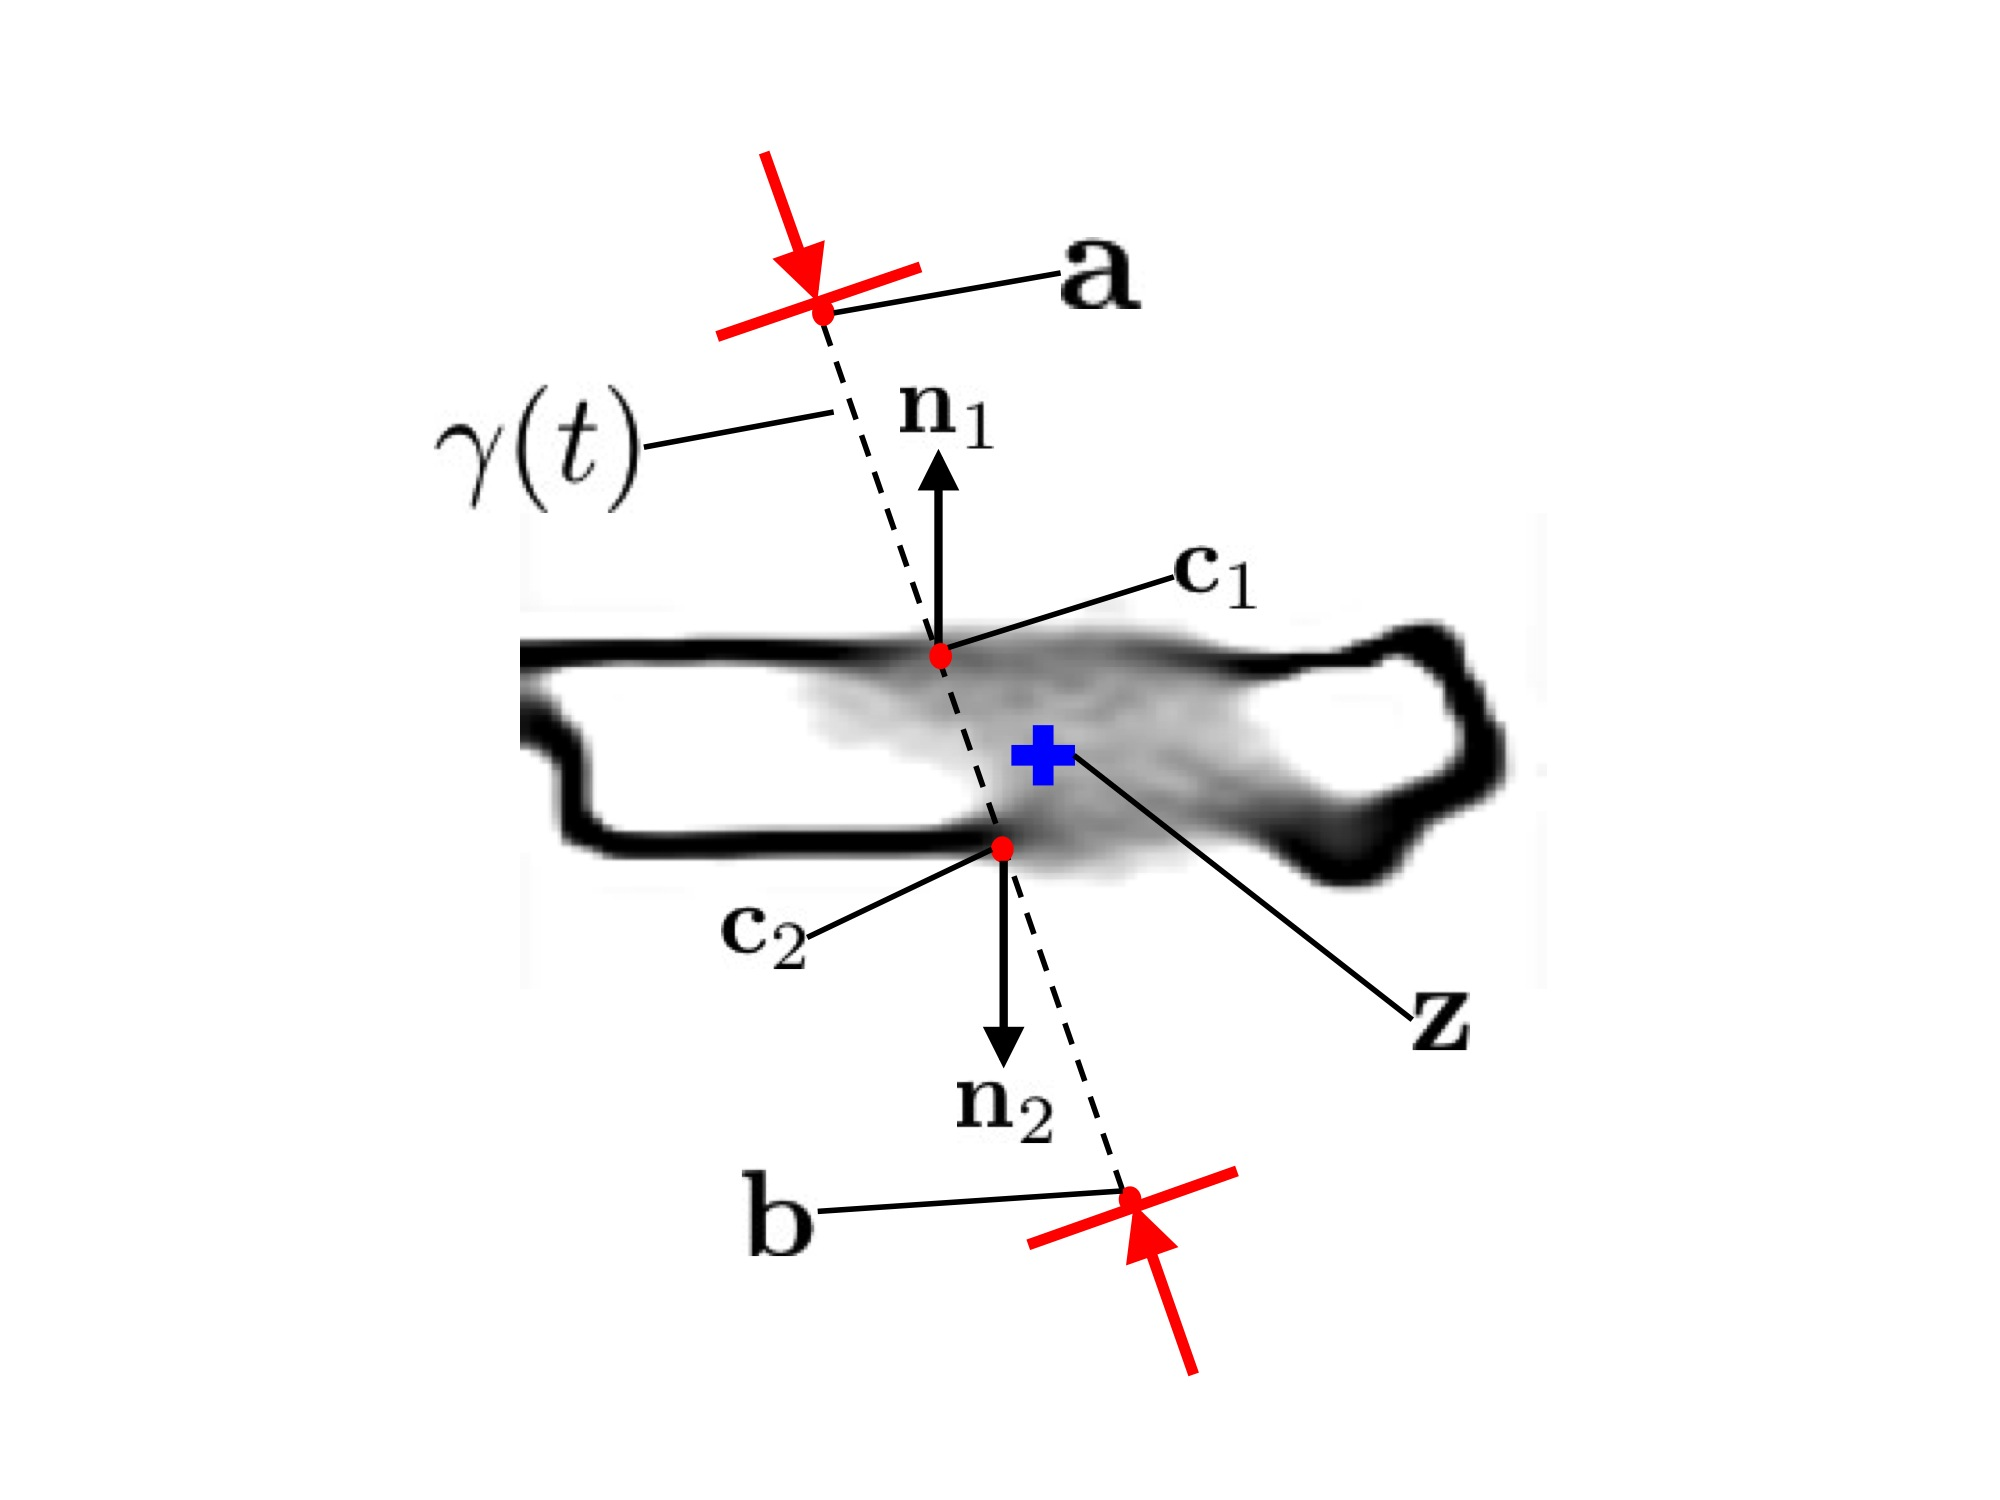
\includegraphics[scale = 0.3]{figures/Slide10.jpg}
\caption{Left: $\epsilon$-greedy policy for sampling (Top 10 grasps plotted)
Right: Monte-Carlo Sampling for 1000 iterations (Top 10 grasps plotted)}
\vspace*{-10pt}
\label{fig:tape_bandit}
\end{figure}

\todo{Write Conclusion}
\bibliographystyle{ieeetr}
\bibliography{references}

\end{document}
